% =====================================================================================
% REVISIÓN 2  -  Propuesta de solución
% Escribe tu texto FUERA de los recuadros \begin{guia} ... \end{guia}.
% =====================================================================================

\section{Propuesta de solución} \label{sec:propuesta} % audit:req=propuesta_solucion

\begin{guia}[Guía: Propuesta de solución (Revisión 2)]
\textbf{¿Para qué sirve?} Explica \emph{qué vas a hacer exactamente y cómo resuelve el problema}, antes de entrar a los
detalles de construcción (Revisión 3).

\textbf{Debe responder:}
\begin{itemize}[nosep,leftmargin=*]
  \item ¿En qué consiste la solución, a grandes rasgos? Incluye un diagrama general (arquitectura, flujo del proceso o
        esquema del método).
  \item \emph{Proyecto de sistema:} ¿cuáles son los requisitos funcionales (qué hará) y no funcionales (rendimiento,
        seguridad, usabilidad)? ¿quiénes son los usuarios y qué roles tienen?
  \item \emph{Proyecto de investigación:} ¿cuál es la hipótesis o pregunta de investigación? ¿qué enfoque o algoritmo
        propones y en qué se diferencia de lo existente?
  \item ¿Qué tecnologías, herramientas y metodología de trabajo usarás y por qué (frente a las alternativas)?
  \item ¿Cómo atiende la propuesta cada objetivo específico? (una tabla ``objetivo $\rightarrow$ componente de la solución''
        es muy útil).
  \item ¿Cuál es el plan de trabajo y el cronograma del cuatrimestre?
  \item ¿Cómo sabrás que funcionó? (criterios de aceptación o métricas de éxito).
\end{itemize}

\textbf{Organización sugerida:} \verb|\subsection| para \emph{Descripción general}, \emph{Requisitos} (o \emph{Hipótesis y
enfoque}), \emph{Tecnologías y metodología} y \emph{Plan de trabajo}.

\textbf{Extensión mínima:} 150 palabras, además de diagramas y tablas.

\textbf{Errores frecuentes:} describir solo tecnologías sin explicar la solución; requisitos vagos (``el sistema será
rápido''); propuesta desconectada de los objetivos; cronograma sin fechas.

\textbf{Cómo se revisa:} coherencia con el problema y los objetivos, viabilidad en un cuatrimestre y claridad técnica.
\end{guia}

% >>> Propuesta de solución: descripción, arquitectura, requisitos, tecnologías y trazabilidad <<<

La solución es un sistema de digitalización inteligente que convierte facturas CFDI, órdenes de compra y remisiones recibidas como PDF o imagen en registros estructurados, validados y consultables mediante API REST. El documento ingresa por un endpoint de carga, atraviesa preprocesamiento de imagen, OCR con confianza por palabra, clasificación por reglas, extracción estructurada con advertencias de integridad y normalización fiscal, y persiste en PostgreSQL con trazabilidad completa de documento, página, campo y confianza\cite{fastapi_docs, tesseract_ocr}.

\subsection{Descripción general y arquitectura del sistema} \label{sec:prop_descripcion}

El sistema se organiza como un pipeline secuencial con persistencia incremental de estado. La Figura~\ref{fig:arquitectura_sistema} resume el flujo: (1)~ingesta por API, (2)~preproceso con OpenCV, (3)~OCR con Tesseract o lectura directa de capa de texto, (4)~clasificación del tipo documental, (5)~extracción estructurada por reglas, (6)~normalización a formas canónicas, (7)~persistencia relacional y (8)~evaluación reproducible con scripts versionados.

\begin{figure}[H]
\centering
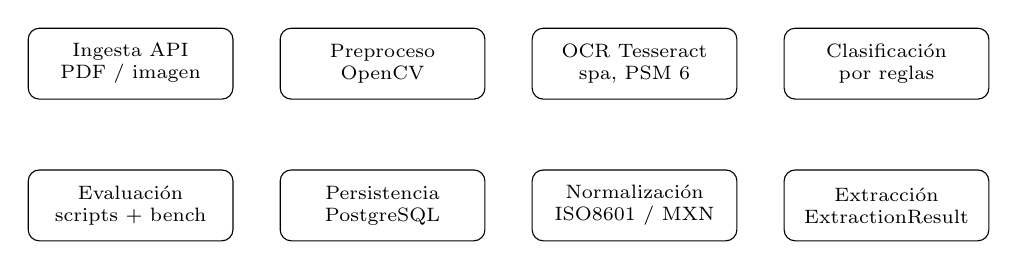
\begin{tikzpicture}[node distance=1.6cm, auto,
  etapa/.style={rectangle, draw, rounded corners, minimum width=2.6cm, minimum height=0.9cm, align=center, font=\scriptsize},
  flecha/.style={->, thick}]
  \node[etapa] (ing) {Ingesta API\\PDF / imagen};
  \node[etapa, right of=ing, node distance=3.2cm] (pre) {Preproceso\\OpenCV};
  \node[etapa, right of=pre, node distance=3.2cm] (ocr) {OCR Tesseract\\spa, PSM 6};
  \node[etapa, right of=ocr, node distance=3.2cm] (cla) {Clasificación\\por reglas};
  \node[etapa, below of=cla, node distance=1.8cm] (ext) {Extracción\\ExtractionResult};
  \node[etapa, left of=ext, node distance=3.2cm] (nor) {Normalización\\ISO8601 / MXN};
  \node[etapa, left of=nor, node distance=3.2cm] (per) {Persistencia\\PostgreSQL};
  \node[etapa, left of=per, node distance=3.2cm] (eva) {Evaluación\\scripts + bench};
  \path[flecha] (ing) -- (pre);
  \path[flecha] (pre) -- (ocr);
  \path[flecha] (ocr) -- (cla);
  \path[flecha] (cla) -- (ext);
  \path[flecha] (ext) -- (nor);
  \path[flecha] (nor) -- (per);
  \path[flecha] (per) -- (eva);
\end{tikzpicture}
\caption{Arquitectura del pipeline: ingesta, preproceso, OCR, clasificación, extracción, normalización, persistencia y evaluación.}
\label{fig:arquitectura_sistema}
\end{figure}

La ingesta recibe el archivo, lo almacena y crea el registro del documento en estado \textit{processing} con tipo provisional \textit{desconocido} y confianza cero; el trabajo pesado se delega a una tarea en segundo plano (\textit{BackgroundTasks}) que ejecuta OCR, clasificación y extracción, y finalmente transiciona el estado a \textit{done} o \textit{error}\cite{fastapi_docs}. El preproceso aplica escala de grises, corrección de inclinación y binarización adaptativa para maximizar el contraste trazo-fondo antes del reconocimiento\cite{bradski_opencv_2008, opencv_docs}. El OCR opera en español con PSM~6 y reporta texto más confianza por palabra; los PDF con capa de texto se leen directamente y los escaneados se renderizan a imagen\cite{tesseract_ocr, smith_tesseract_2007}. La clasificación asigna \textit{factura}, \textit{orden\_compra}, \textit{remision} o \textit{desconocido} mediante reglas lexicales inspeccionables\cite{sokolova_metrics_2009}. La extracción produce el objeto \textit{ExtractionResult} con folio, fecha, RFC de emisor y receptor, UUID, conceptos y totales, emitiendo la advertencia \textit{TOTALS\_MISMATCH} cuando los montos no cuadran\cite{structured_extraction_2023}. La normalización fija fechas a ISO~8601, montos a decimal en MXN y cadenas fiscales a su forma canónica antes de validar con Pydantic~v2 y persistir con SQLAlchemy\cite{pydantic_v2_2024, sqlalchemy_docs_2024}. La evaluación corre sobre 30 documentos oficiales más 4 excluidos documentados, con scripts de evaluación y de medición de latencias\cite{structured_extraction_2023, sokolova_metrics_2009}.

\subsection{Requisitos funcionales y no funcionales} \label{sec:prop_requisitos}

Los requisitos funcionales describen lo que el sistema hace; los no funcionales, las propiedades con que debe hacerlo. Ambos se verifican contra los objetivos en la Sección~\ref{sec:prop_trazabilidad}.

\begin{table}[H]
\centering
\small
\caption{Requisitos funcionales del sistema.}
\label{tab:requisitos_funcionales}
\begin{tabular}{@{}p{2.8cm}p{10.7cm}@{}}
\toprule
\textbf{Identificador} & \textbf{Descripción} \\
\midrule
RF-01 & Cargar documentos en PDF o imagen mediante un endpoint dedicado, almacenar el archivo y registrar sus metadatos con validación tipada\cite{fastapi_docs, pydantic_v2_2024}. \\
RF-02 & Preprocesar la imagen con escala de grises, corrección de inclinación y binarización adaptativa antes del OCR\cite{bradski_opencv_2008, opencv_docs}. \\
RF-03 & Extraer texto con Tesseract en español y PSM~6, con confianza por palabra; leer directamente la capa de texto de los PDF que la posean\cite{tesseract_ocr, smith_tesseract_2007}. \\
RF-04 & Clasificar cada documento como factura, orden\_compra, remision o desconocido mediante reglas lexicales auditables\cite{sokolova_metrics_2009}. \\
RF-05 & Extraer campos estructurados (folio, fecha, RFC de emisor y receptor, UUID, conceptos, impuestos, total) en un objeto \textit{ExtractionResult} con advertencias de integridad, incluida \textit{TOTALS\_MISMATCH}\cite{structured_extraction_2023}. \\
RF-06 & Normalizar fechas a ISO~8601, montos a decimal en MXN y cadenas fiscales a su forma canónica\cite{pydantic_v2_2024}. \\
RF-07 & Persistir documentos, páginas, campos y resultados en PostgreSQL con trazabilidad de documento, página, campo y confianza\cite{postgres_docs_2024, sqlalchemy_docs_2024}. \\
RF-08 & Exponer carga, consulta y recuperación de resultados mediante API REST documentada, con procesamiento asíncrono (\textit{processing}, \textit{done}, \textit{error}) y esquemas validados\cite{fielding_rest_2000, fastapi_docs}. \\
\bottomrule
\end{tabular}
\end{table}

\begin{table}[H]
\centering
\small
\caption{Requisitos no funcionales del sistema.}
\label{tab:requisitos_no_funcionales}
\begin{tabular}{@{}p{2.8cm}p{10.7cm}@{}}
\toprule
\textbf{Identificador} & \textbf{Descripción} \\
\midrule
RNF-01 & Exactitud: al menos 90\% en RFC, UUID y totales, y al menos 80\% en conceptos y órdenes de compra, medidos por campo con tolerancia de $\pm 1.00$ en montos (umbrales de diseño; verificación empírica en fase de pruebas)\cite{sokolova_metrics_2009}. \\
RNF-02 & Validez del contrato: 100\% de respuestas del pipeline conformes al esquema \textit{ExtractionResult} (tasa de JSON válido)\cite{pydantic_v2_2024}. \\
RNF-03 & Latencia de reglas: la etapa de clasificación y extracción sobre texto limpio opera en el orden de décimas de milisegundo (referencia medida: p50 de 0.08~ms y p95 de 0.09~ms); el OCR queda fuera de este presupuesto por depender del motor y de la imagen\cite{sokolova_metrics_2009}. \\
RNF-04 & Ejecución local en CPU sin GPU y sin costo por documento, con tecnologías abiertas auditables\cite{tesseract_ocr, docker_docs}. \\
RNF-05 & Reproducibilidad: entorno completo contenerizado (API más base de datos) con verificaciones de salud y volúmenes persistentes\cite{docker_docs}. \\
RNF-06 & Confidencialidad: los comprobantes fiscales permanecen en la infraestructura local; no se envían a servicios externos\cite{sat_cfdi_2024, gcp_document_ai}. \\
RNF-07 & Trazabilidad: todo campo persistido conserva su documento, página y confianza de reconocimiento de origen\cite{postgres_docs_2024}. \\
\bottomrule
\end{tabular}
\end{table}

Los usuarios del sistema son el personal administrativo que carga y verifica documentos, el auditor que consulta la trazabilidad por campo y los sistemas consumidores (por ejemplo, el frontend del equipo) que integran los resultados mediante el contrato tipado de la API\cite{fielding_rest_2000, fastapi_docs}.

\subsection{Tecnologías elegidas y alternativas descartadas} \label{sec:prop_tecnologias}

La Tabla~\ref{tab:decision_tecnologica} resume cada decisión frente a su alternativa principal. El criterio transversal es triple: ejecución local auditable, especificidad fiscal mexicana y reproducibilidad del entorno.

\begin{table}[H]
\centering
\small
\caption{Decisiones tecnológicas frente a alternativas.}
\label{tab:decision_tecnologica}
\begin{tabular}{@{}p{2.6cm}p{3.6cm}p{3.6cm}p{3.6cm}@{}}
\toprule
\textbf{Aspecto} & \textbf{Tecnología elegida} & \textbf{Alternativa} & \textbf{Justificación} \\
\midrule
Framework web & FastAPI (enrutadores tipados, tareas en segundo plano, documentación automática) & Flask o Django & FastAPI integra validación tipada y asincronía nativa para el worker de OCR; Flask exigiría ensamblarlas manualmente y Django aporta un monolito innecesario para una API de pipeline\cite{fastapi_docs}. \\
Validación & Pydantic~v2 estricto (RFC, UUID, ISO~8601, rangos) & Dataclasses o validación manual & El contrato se vuelve ejecutable: los datos se rechazan antes de persistir y la tasa de JSON válido es medible; las dataclasses no validan formatos ni rangos\cite{pydantic_v2_2024}. \\
Persistencia & PostgreSQL~16 con SQLAlchemy & SQLite & PostgreSQL aporta ACID con concurrencia multiversión, tipos estrictos e índices para folio, RFC y UUID en operación concurrente; SQLite no sostiene dicho régimen multiusuario\cite{postgres_docs_2024, sqlalchemy_docs_2024}. \\
OCR & Tesseract local (spa, PSM~6, confianza por palabra) & Servicios en la nube & Tesseract elimina el costo por documento, mantiene los comprobantes en la infraestructura local y permite auditar cada etapa; la nube ofrece mayor exactitud base a cambio de costo, dependencia externa y salida de datos fiscales\cite{tesseract_ocr, gcp_document_ai}. \\
Despliegue & Docker Compose (api más db, \textit{healthchecks}, volúmenes) & Instalación directa en el sistema & Compose fija el entorno evaluado (Tesseract con español, OpenCV, PostgreSQL~16) y lo hace reproducible en cualquier máquina; la instalación directa acopla la medición a la máquina del desarrollador\cite{docker_docs}. \\
\bottomrule
\end{tabular}
\end{table}

La metodología de trabajo es iterativa por incrementos verificables: cada etapa del pipeline (ingesta, preproceso, OCR, clasificación, extracción, persistencia, evaluación) se implementa con su script de verificación correspondiente, de modo que ningún incremento se declara concluido sin evidencia de ejecución sobre el conjunto documental\cite{structured_extraction_2023}.

\subsection{Trazabilidad a objetivos específicos y criterios de aceptación} \label{sec:prop_trazabilidad}

La Tabla~\ref{tab:trazabilidad_objetivos} vincula cada objetivo específico (Sección~\ref{subsec:objetivos_especificos}) con el componente que lo realiza, los requisitos que lo verifican y la evidencia que demuestra su cumplimiento.

\begin{table}[H]
\centering
\small
\caption{Trazabilidad objetivo, componente, requisito y verificación.}
\label{tab:trazabilidad_objetivos}
\begin{tabular}{@{}p{1.9cm}p{3.2cm}p{2.2cm}p{5.7cm}@{}}
\toprule
\textbf{Objetivo} & \textbf{Componente} & \textbf{Requisitos} & \textbf{Verificación} \\
\midrule
OE-1: endpoint de carga & Ingesta API & RF-01, RF-08 & Carga de PDF e imagen con metadatos persistidos; contrato validado (RNF-02)\cite{fastapi_docs}. \\
OE-2: preprocesamiento & Preproceso OpenCV & RF-02 & Documentos enderezados y binarizados antes del OCR; parámetros calibrados sobre el conjunto\cite{opencv_docs}. \\
OE-3: OCR Tesseract & Motor OCR & RF-03 & Texto con confianza por palabra; capa de texto tratada sin OCR y escaneados renderizados a imagen\cite{tesseract_ocr}. \\
OE-4: clasificador por reglas & Clasificación & RF-04 & Exactitud por clase sobre el conjunto; clase \textit{desconocido} para formatos inéditos\cite{sokolova_metrics_2009}. \\
OE-5: esquema relacional & Persistencia & RF-07 & Trazabilidad documento--página--campo--confianza en PostgreSQL (RNF-07)\cite{postgres_docs_2024}. \\
OE-6: API REST tipada & Backend FastAPI más Pydantic & RF-08, RF-06 & Documentación interactiva y 100\% de JSON válido contra \textit{ExtractionResult}\cite{pydantic_v2_2024}. \\
OE-7: protocolo de evaluación & Scripts evaluar y bench & RF-05, RNF-01--RNF-03 & Exactitud por campo con $\pm 1.00$ en montos; 100\% en reglas sobre texto limpio con p50 de 0.08~ms; OCR real pendiente del entorno Docker\cite{sokolova_metrics_2009}. \\
OE-8: contenerización & Docker Compose & RNF-04, RNF-05 | RNF-06 & Despliegue api más db con \textit{healthchecks}; datos fiscales sin salida externa\cite{docker_docs}. \\
\bottomrule
\end{tabular}
\end{table}

El plan de trabajo del cuatrimestre sigue el orden del pipeline: primero ingesta y persistencia, después preproceso y OCR, luego clasificación y extracción con normalización, y finalmente contenerización y evaluación completa. El criterio global de aceptación es que los ocho objetivos presenten su evidencia de verificación: endpoints operativos, documentos procesados de extremo a extremo, métricas por campo reportadas con su protocolo y entorno Docker reproducible\cite{structured_extraction_2023, docker_docs}. La medición con OCR real sobre documentos escaneados, pendiente del entorno Docker completo, y la extracción asistida por modelo multimodal, correspondiente a una fase siguiente\cite{kim_donut_2022}, quedan explícitamente fuera del criterio de aceptación del presente avance.

% EVIDENCIA: fastapi_docs --- anexar impresión de la guía de BackgroundTasks y validación de esquemas con fecha de consulta.
% EVIDENCIA: docker_docs --- anexar impresión de la guía de Compose (depends_on con healthcheck, volúmenes) con fecha de consulta.
% EVIDENCIA: sokolova_metrics_2009 --- anexar definiciones de precisión, cobertura, F y promedio macro aplicadas al protocolo por campo.
